\documentclass[
11pt,notheorems,hyperref={pdfauthor=Jakob}
]{beamer}

\input{loadslides.tex}

\title[Replication Project]{Democratic Sanctions and the Selective Targeting of Authoritarian Regimes}
\subtitle{Replication and Extension Presentation}
\author[Jakob]{Jakob Lütkemeier}
\institute{M.Sc. Applied Social Data Science \\ Trinity College Dublin}
\date{Applied Statistical Analysis II}

% Pass 1 placeholder utility
\newcommand{\placeholderbox}[2]{%
	\begin{center}
		\setlength{\fboxsep}{10pt}%
		\fbox{%
			\begin{minipage}[c][#2][c]{0.86\linewidth}
				\centering
				\textbf{#1}
			\end{minipage}%
		}
	\end{center}
}

\begin{document}
	
	{
		\setbeamertemplate{footline}{}
		\begin{frame}
			\titlepage
		\end{frame}
	}
	\addtocounter{framenumber}{-1}
	
	\section{Puzzle and Argument}
	
	\begin{frame}{Why are some dictators sanctioned and others spared?}
		\begin{itemize}
			\item Democratic sanctions are meant to punish authoritarian backsliding.
			\item Yet many authoritarian regimes violate democratic norms without being sanctioned.
			\item Others are sanctioned quickly after visible political shocks.
			\item \textit{Example.} Belarus 2020 vs Bahrain 2011: similar authoritarian backsliding, but only Belarus faced broad Western sanctions.
		\end{itemize}
		
		\vspace{0.5em}
		
		\begin{alertblock}{Core puzzle}
			If sanctions are not simply a reaction to repression, what other factors are at play?
		\end{alertblock}
	\end{frame}
	
\begin{frame}{The paper's answer}{A three-part framework}
	\begin{columns}[T,onlytextwidth]
		\column{0.32\textwidth}
		\begin{block}{Trigger}
			\begin{itemize}
				\item Coups
				\item Controversial elections
			\end{itemize}
		\end{block}
		
		\column{0.32\textwidth}
		\begin{block}{Target vulnerability}
			\begin{itemize}
				\item Weaker regimes
				\item Less resilient targets
			\end{itemize}
		\end{block}
		
		\column{0.32\textwidth}
		\begin{block}{Sender costs}
			\begin{itemize}
				\item Economic exposure
				\item Political alignment
			\end{itemize}
		\end{block}
	\end{columns}
	
	\vspace{0.5em}
	
	\begin{exampleblock}{Main Hypothesis}
		Democratic sanctions depend not only on trigger events, but also on target vulnerability and sender costs.
	\end{exampleblock}
\end{frame}
	
	\section{Replication}
	
	\begin{frame}{What exactly I replicated}
		\begin{columns}[T,onlytextwidth]
			\column{0.56\textwidth}
			\begin{block}{Design}
				\begin{itemize}
					\item Unit of analysis: authoritarian \textbf{country-years}
					\item Time window: 1990--2010
					\item Outcome: \textbf{democratic sanction onset} (binary).
					\item Main estimator: \textbf{clustered logit} for binary onset
				\end{itemize}
			\end{block}
			
			\column{0.38\textwidth}
			\begin{block}{Replicated outputs}
				\begin{itemize}
					\item Table I
					\item Table II
					\item Table III
					\item Figure 2
				\end{itemize}
			\end{block}
		\end{columns}
		
		\vspace{0.4em}
		
		\begin{exampleblock}{What is a \textit{clustered} logit model?}
			Like normal logit, a clustered logit models the probability of a binary outcome. The difference is that it adjusts the standard errors because repeated observations from the same country are likely correlated.
		\end{exampleblock}

	\end{frame}
	
	\begin{frame}{Replication result}{Dramatic triggers matter most}
		\begin{columns}[T,onlytextwidth]
			\column{0.43\textwidth}
			\begin{itemize}
				\item The replication recovers the paper's \textbf{trigger hierarchy}.
				\item \textbf{Coups} sharply increase sanction likelihood.
				\item \textbf{Controversial elections} also matter, but less strongly.
				\item Static democratic weakness is less important than visible political shocks.
			\end{itemize}
			
			\vspace{0.4em}
			\begin{block}{Interpretation}
				Sanctions respond most strongly to events that are politically visible and difficult to ignore.
			\end{block}
			
			\column{0.53\textwidth}
			\begin{block}{\centering \footnotesize Table I: trigger coefficients}
				\centering
				\scriptsize
				\begin{tabular}{lccc}
					\hline
					& Western & EU & US \\
					\hline
					Coup & 5.127*** & 3.765*** & 4.947*** \\
					Democracy score & $-0.056$ & $-0.081$ & $-0.116$ \\
					Controversial election & 2.584*** & 2.620*** & 2.275*** \\
					\hline
				\end{tabular}
			\end{block}
			
			\vspace{0.3em}
			
			\begin{block}{\centering \footnotesize Table II: predicted probabilities}
				\centering
				\scriptsize
				\begin{tabular}{lccc}
					\hline
					& Western & EU & US \\
					\hline
					Baseline & 0.007 & 0.007 & 0.004 \\
					Coup & 0.519 & 0.232 & 0.346 \\
					Controversial election & 0.074 & 0.084 & 0.032 \\
					\hline
				\end{tabular}
			\end{block}
		\end{columns}
	\end{frame}
	
	\begin{frame}{Replication result}{Sanctions are selective, not automatic}
		\begin{columns}[T,onlytextwidth]
			\column{0.43\textwidth}
		\begin{itemize}
			\item Sanctions are not explained by triggers alone.
			\item \textbf{Target vulnerability} matters: higher \textbf{inflation} is associated with higher sanction odds.
			\item \textbf{Sender costs} matter: politically closer regimes and regimes with higher \textbf{FDI} are less likely to be sanctioned.
		\end{itemize}
			\vspace{0.4em}
			\begin{block}{Interpretation}
				Even when democratic violations occur, sanctions depend on both \textbf{target vulnerability} and \textbf{sender costs}.
			\end{block}
			
			\column{0.53\textwidth}
			\begin{block}{\centering \footnotesize Table III: selective-targeting coefficients}
				\centering
				\scriptsize
				\begin{tabular}{lc}
					\hline
					& Western \\
					\hline
					Coup & 5.128*** \\
					Controversial election & 2.909*** \\
					Inflation ($t-1$) & 0.022** \\
					FDI inflows ($t-1$) & $-0.046$* \\
					Political closeness to West ($t-1$) & $-4.413$** \\
					\hline
				\end{tabular}
			\end{block}
		\end{columns}
	\end{frame}
	
	\begin{frame}{Replication results}{When sender costs matter most}
		\begin{block}{Controversial election $\times$ FDI }
			Table III shows that \textbf{sender costs} matter on average. Figure 2 shows \emph{when} one sender-cost variable---\textbf{FDI}---matters most: after \textbf{controversial elections}.
		\end{block}
		
		\vspace{0.4em}
		\begin{figure}
			\centering
			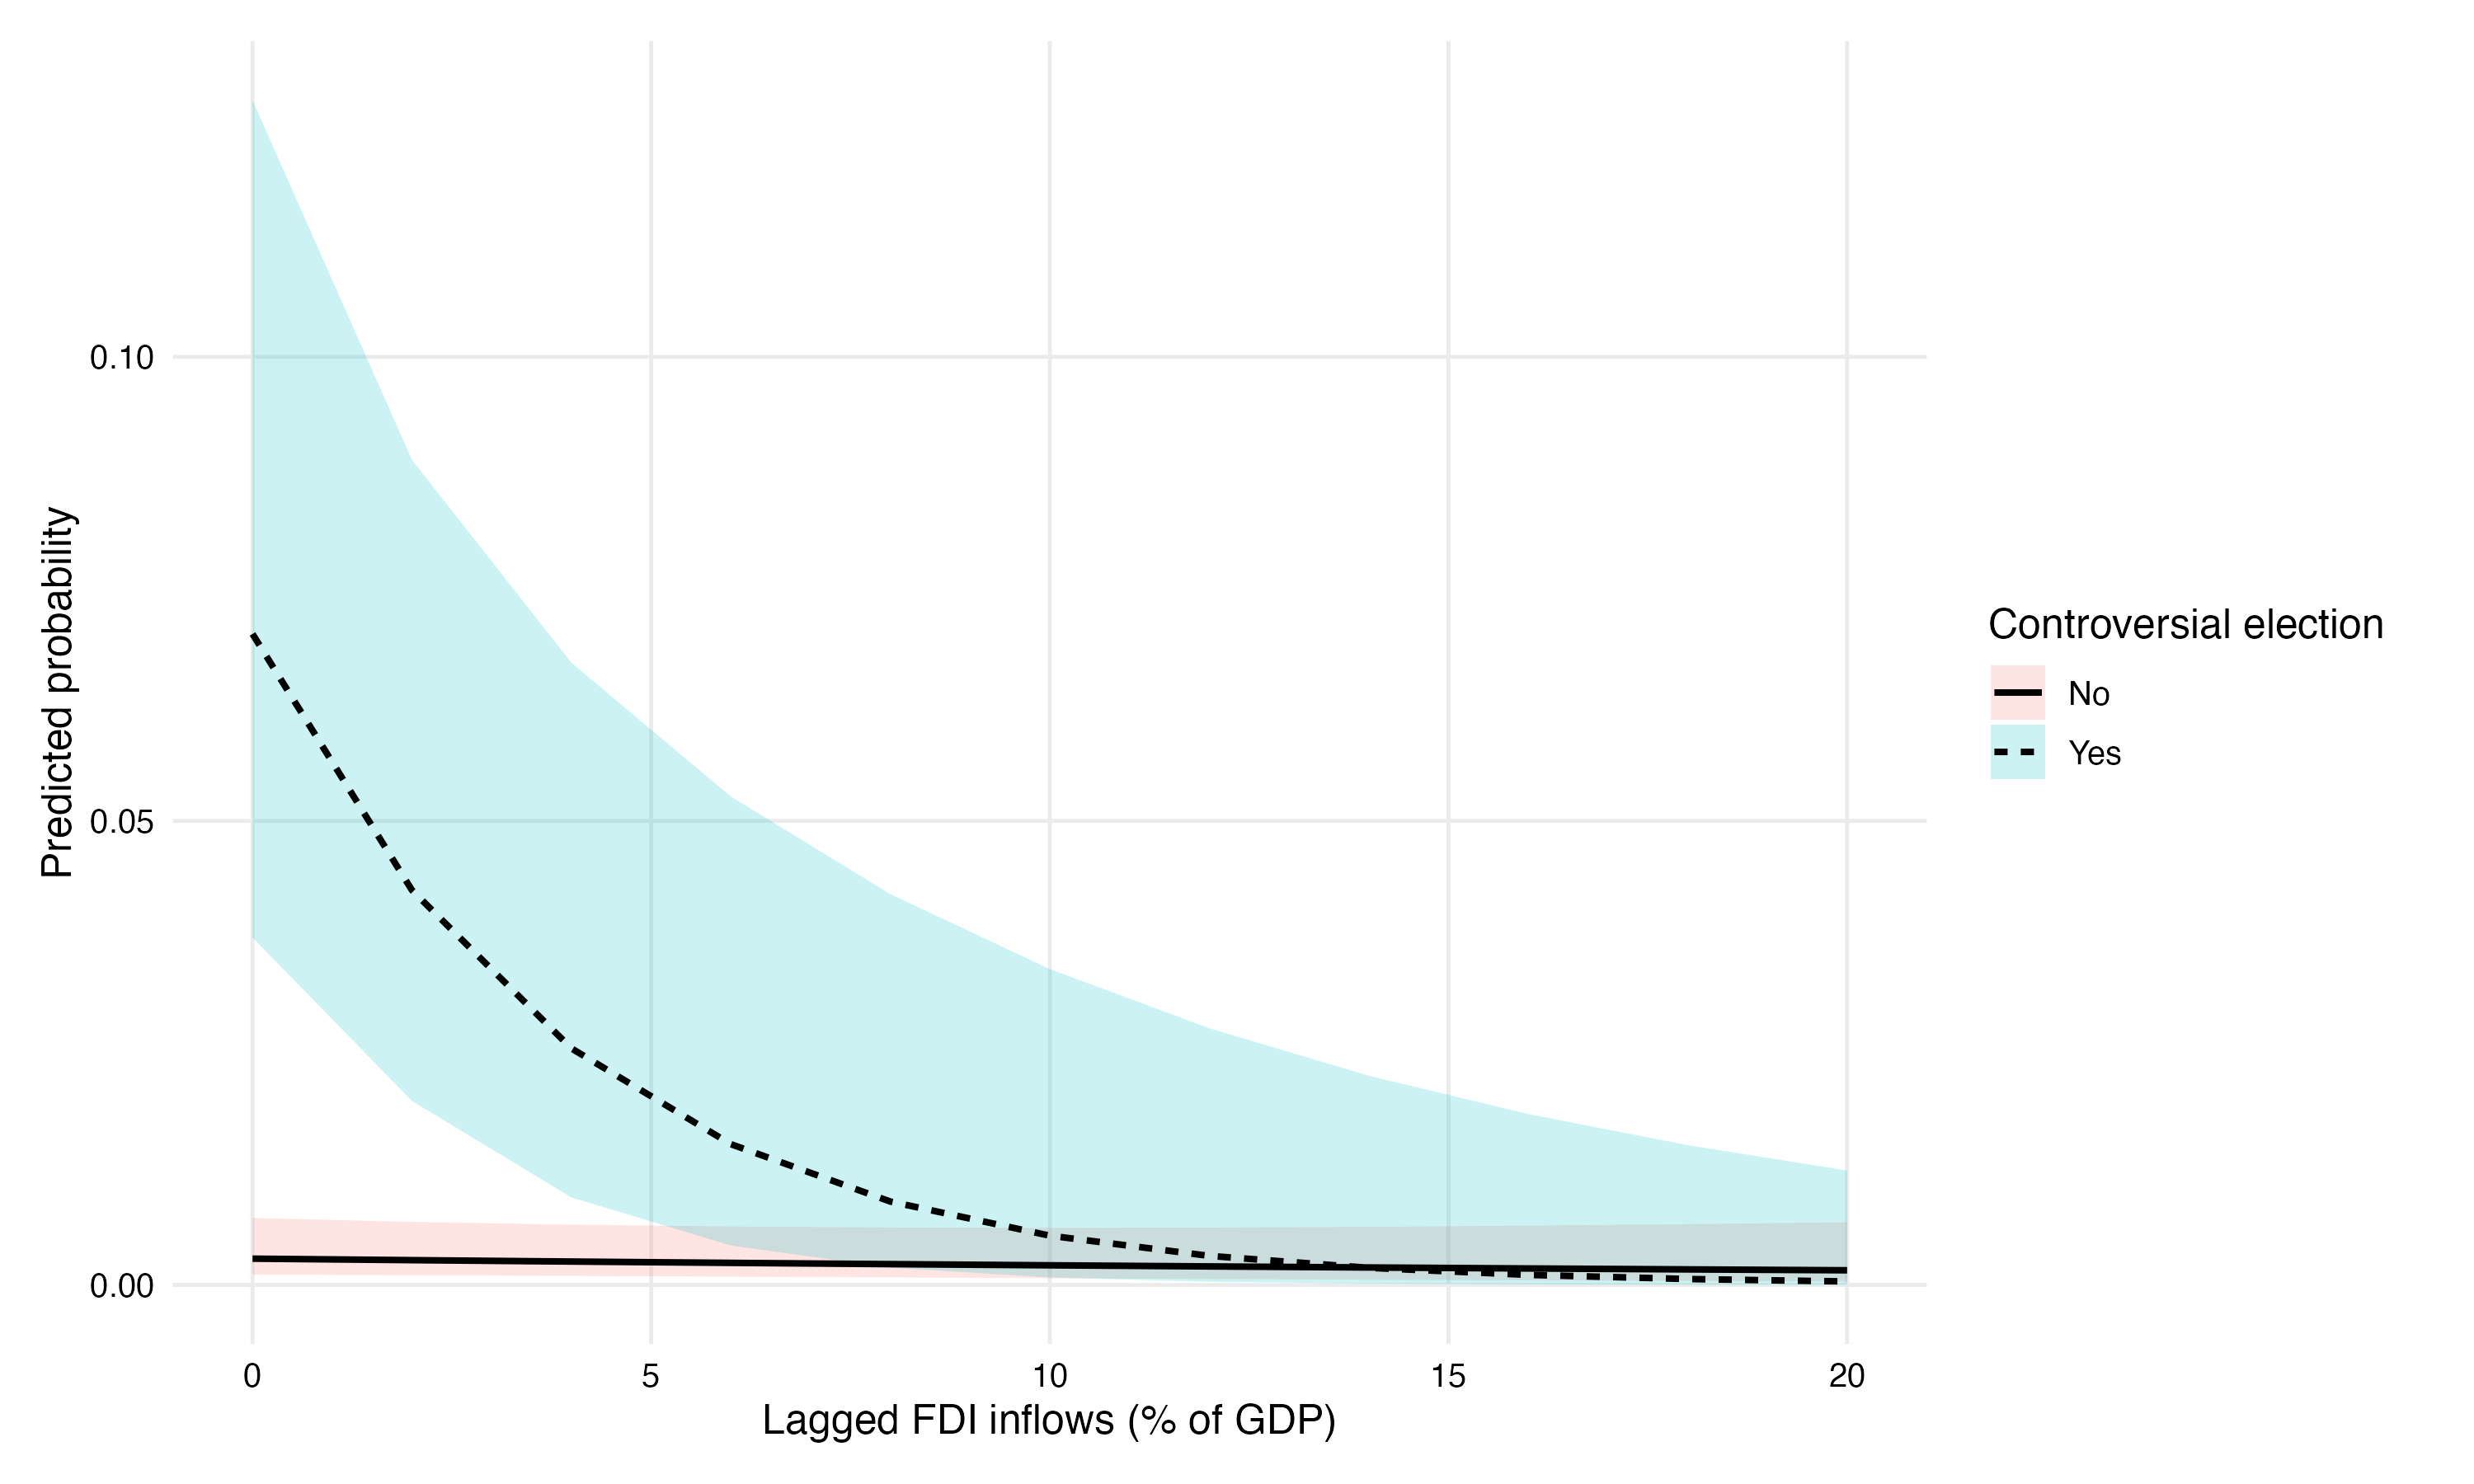
\includegraphics[width=0.7\linewidth]{figures/figure_2_fdi_by_election_status.png}
		\end{figure}

	\end{frame}
	
	\section{Extension}
	
	\begin{frame}{My extension}{Does geopolitical alignment also shield regimes?}
		\begin{alertblock}{Extension question}
			If economic exposure can shield regimes after weaker triggers, can \textbf{political alignment} do the same?
		\end{alertblock}
		
		\vspace{0.4em}
		
		\begin{columns}[T,onlytextwidth]
			\column{0.52\textwidth}
			\begin{block}{Motivation}
				\begin{itemize}
					\item The paper already shows that political closeness matters overall.
					\item Figure 2 suggests discretion is greatest after controversial elections.
					\item The natural next step is to test whether political alignment matters \emph{especially there}.
				\end{itemize}
			\end{block}
			
			\column{0.42\textwidth}
			\begin{block}{Setup}
				\begin{itemize}
					\item Controversial Election $\times$ High Political Closeness
					\item High Closeness = top quartile of UN voting similarity.
					\item Coded as a dummy: 1 = top quartile,\\ 0 = lower three quartiles.
				\end{itemize}
			\end{block}
		\end{columns}
	\end{frame}
	
	\begin{frame}{Extension result}{The pattern is there, but cautiously}
		\begin{columns}[T,onlytextwidth]
			\column{0.44\textwidth}
			\begin{itemize}
				\item Descriptively, controversial elections are followed by \textbf{fewer sanctions} among highly aligned regimes.
				\item The interaction term is \textbf{negative}, matching the theoretical expectation.
				\item The direction is substantively interesting, but the evidence is not strong enough to present as decisive.
			\end{itemize}
			
			\vspace{0.4em}
			\begin{block}{Verdict}
				Theory-consistent and informative, but inferentially uncertain.
			\end{block}
			
			\column{0.52\textwidth}
			\begin{block}{\centering \footnotesize Extension model: interaction coefficients}
				\centering
				\scriptsize
				\begin{tabular}{lcc}
					\hline
					& Baseline & Interaction \\
					\hline
					Controversial election & 2.817*** & 3.123*** \\
					High political closeness (top quartile) & $-1.295$+ & $-0.590$ \\
					Controversial election $\times$ high political closeness &  & $-1.784$ \\
					\hline
				\end{tabular}
			\end{block}
			
			\vspace{0.3em}
			
			\begin{block}{\centering \footnotesize Observed sanction rates by political closeness}
				\centering
				\scriptsize
				\begin{tabular}{lccc}
					\hline
					Political closeness & $N$ & Sanctions & Rate \\
					\hline
					Lower 3 quartiles & 59 & 10 & 0.169 \\
					Top quartile & 44 & 1 & 0.023 \\
					\hline
				\end{tabular}
			\end{block}
		\end{columns}
	\end{frame}
		
	\begin{frame}{Extension robustness checks}
		\begin{itemize}
			\item I varied the threshold used to define \textbf{high political closeness}.
			\item The interaction remained \textbf{negative} under nearby one-year threshold choices.
			\item With a \textbf{two-year lag} of political closeness, the interaction weakened and lost directional consistency.
			\item Overall, the extension is \textbf{plausible but specification-sensitive}.
		\end{itemize}
		
		\vspace{0.6em}
		\begin{block}{Takeaway}
			The robustness checks support a cautious reading: the extension is theory-consistent and informative, but not decisive.
		\end{block}
	\end{frame}
		
	\section{Conclusion}
	
	\begin{frame}{Takeaway}{Strong replication, modest extension}
		\begin{columns}[T,onlytextwidth]
			\column{0.48\textwidth}
			\begin{block}{Replication}
				\begin{itemize}
					\item Core findings are successfully recovered.
					\item Coups and controversial elections matter.
					\item Sender costs \& target vulnerability are central.
				\end{itemize}
			\end{block}
			
			\column{0.48\textwidth}
			\begin{block}{Extension}
				\begin{itemize}
					\item Political alignment may also shield regimes.
					\item Most plausibly after weaker triggers.
					\item Evidence is suggestive, not definitive.
				\end{itemize}
			\end{block}
		\end{columns}
		
		\vspace{0.5em}
		\begin{alertblock}{Final message}
			Democratic sanctions are \textbf{selective}: they reflect not only authoritarian violations, but also target vulnerability and the strategic costs faced by sanctioning states.
		\end{alertblock}
	\end{frame}
	
\end{document}